\documentclass[11pt,a4paper]{article}
\usepackage[T1]{fontenc}
\usepackage[utf8]{inputenc}
\usepackage{amsmath,amssymb,amsthm}
\usepackage[margin=2.6cm]{geometry}
\usepackage{booktabs}
\usepackage{graphicx}
\graphicspath{{figs/}{../figs/}}
\usepackage[colorlinks=true,linkcolor=black,citecolor=black,urlcolor=black]{hyperref}

\renewcommand{\theequation}{N.\arabic{equation}}
\newcommand{\R}{\mathbb{R}}
\newcommand{\E}{\mathbb{E}}
\newcommand{\KL}{\mathrm{KL}}
\newcommand{\DEP}{\mathrm{DEP}}
\newcommand{\diag}{\operatorname{diag}}
\newcommand{\Neff}{N_{\mathrm{eff}}}
\newcommand{\dd}{\mathrm{d}}

\title{\large\bfseries Appendice numerica: un ambiente one-asset minimale per la diagnostica entropica\\[2pt]
\normalsize\itshape materiale di accompagnamento all'integrazione tecnica (equazioni I.1--I.15) della nota\\ \emph{Diagnostica entropica delle dinamiche distributive nei modelli HANK}}
\author{\normalsize Francesco Pinna}
\date{\normalsize 11 giugno 2026}

\renewcommand{\figurename}{Figura}
\renewcommand{\tablename}{Tabella}
\renewcommand{\abstractname}{Sommario}

\begin{document}
\maketitle

\begin{abstract}
\noindent Il presente documento esercita su un ambiente one-asset, risolto in modo esatto e senza alcuna componente stimata, l'intera pipeline (I.15) dell'integrazione tecnica: dizionario di tilt regionali (I.6), prior idiosincratico fissato dal pinning (I.10), decomposizione esatta del costo (I.11), legge weighted-$\chi^2$ del null direzionale (I.13) con p-value calcolati per quadratura di Imhof, capacit\`a e direzioni massimamente confondenti (Definizione 10.1), matrice di confusione pre-dati e risoluzione diagnostica (Definizione 10.2), controlli C1--C3 nella forma analitica. Tutte le identit\`a teoriche risultano verificate ai limiti della precisione di macchina. L'esercizio restituisce per\`o alla teoria quattro risultati sostanziali, che il documento argomenta e quantifica. Nello specifico, il confronto fra layer aggregato e idiosincratico richiede una taglia effettiva del panel $\Neff$ che la convenzione per capita del Lemma 9.1 lascia indeterminata, i p-value marginali della (I.13) saturano congiuntamente su segnali forti e il rimedio pairwise dell'Osservazione 10.6 \`e sistematicamente distorto verso i blocchi ad alta capacit\`a; la statistica di attribuzione corretta \`e la frazione di capacit\`a utilizzata $u_k=s_k/\lambda_{\max}^{(k)}$, che emenda la Definizione 10.2, la risoluzione della famiglia annidata non \`e monotona nel raffinamento ed \`e strettamente crescente nell'insieme dei momenti vincolati, sicch\'e la risoluzione \`e una propriet\`a congiunta della coppia dizionario--momenti e non del solo dizionario.
\end{abstract}

\section{Oggetto e sintesi dei risultati}
La funzione di questo esercizio è quella di stabilire che ogni oggetto della pipeline sia calcolabile, che le identit\`a esatte tengano numericamente, e soprattutto sottoporre a stress le parti del disegno che la teoria lascia sottodeterminate, ossia la scala relativa dei prior fra layer, il comportamento dei p-valori in regime di segnale forte, la regola di attribuzione e la semantica della risoluzione. Su un modello deliberatamente minimale ciascuno di questi punti pu\`o essere isolato senza ambiguit\`a, perch\'e gli esperimenti di iniezione sono controllati: la verit\`a \`e nota per costruzione.

Quattro risultati retroagiscono sulla teoria, e sono discussi nelle Sezioni \ref{sec:neff}, \ref{sec:confusione}, che ne raccoglie due, e \ref{sec:risoluzione}. Il primo riguarda la scala fra i due livelli della diagnostica. Con la sola convenzione per capita della (I.10), deformare il livello idiosincratico risulta quasi gratuito in termini informativi, al punto che la capacit\`a del blocco aggregato scende a $0{,}002$ e ogni residuo viene attribuito al churn, sicch\'e il pinning va completato con una taglia effettiva $\Neff$ del panel, che va dichiarata come statistica del disegno empirico.
Il secondo è legato la molteplicit\`a. Con maggior dettaglio, per segnali forti, i p-value marginali della (I.13) saturano sotto $10^{-12}$ su pi\`u blocchi contemporaneamente, come anticipato dall'Osservazione 10.6, ma il rimedio proposto in quella sede, basato sui contrasti a coppie, risulta distorto verso i blocchi ad alta capacit\`a e sbaglia l'attribuzione anche su residui perfettamente lineari, il che esclude l'errore di linearizzazione e riconduce il fallimento a un confondimento strutturale.
Il terzo individua la regola che ripara questo difetto. Infatti in tutti i casi in cui i contrasti a coppie falliscono, attribuisce correttamente la frazione di capacit\`a utilizzata $u_k=s_k/\lambda_{\max}^{(k)}$, un corollario immediato della Definizione 10.1 che propongo di promuovere a regola di attribuzione nella Definizione 10.2, lasciando ai p-value il solo giudizio di significativit\`a sul blocco attribuito.
Il quarto risultato riguarda infine la risoluzione della famiglia annidata $K\in\{1,2,4,8\}$, che non \`e monotona nel raffinamento. Sui soli momenti aggregati la partizione con $K=1$ fallisce, quella con $K=2$ risolve, quella con $K=4$ risolve con un margine trascurabile e quella con $K=8$ fallisce, mentre l'aggiunta di dodici momenti sul consumo della met\`a meno ricca della popolazione porta da $K=2$ a $K=4$ la partizione pi\`u fine risolta con margine apprezzabile e sblocca anche $K=1$. La risoluzione \`e dunque una propriet\`a congiunta del dizionario e dei momenti, e la Definizione 10.2 va indicizzata a entrambi.

\section{Ambiente, dizionario e convenzioni}\label{sec:ambiente}
Il modello \`e il blocco consumo--risparmio di un'economia alla Aiyagari in equilibrio parziale, a tempo discreto trimestrale. Le famiglie hanno utilit\`a CRRA con avversione $\gamma=2$ e fattore di sconto $\beta=0{,}97$, il reddito da lavoro segue una catena a due stati $y\in\{0{,}70;\,1{,}30\}$ con matrice baseline simmetrica di persistenza $0{,}925$, il tasso reale \`e $r=0{,}01$, il vincolo $a\ge0$ su una griglia di $120$ punti a spaziatura potenza $2{,}5$ su $[0,60]$. La politica \`e risolta con endogenous grid method e la misura evolve con i pesi a lotteria di Young. Più precisamente, lo stazionario presenta consumo aggregato $C=1{,}0151$, ricchezza aggregata $A=1{,}5082$ e una massa al vincolo pari a $0{,}1913$. L'orizzonte di troncamento \`e $T=40$ trimestri; il vettore base dei momenti raccoglie $H=24$ deviazioni percentuali del consumo aggregato, $m_t=100\,\dd C_t/C_{ss}$ per $t=0,\dots,23$.

Il dizionario \`e l'istanza pi\`u semplice della (I.6). Qui il tilt agisce moltiplicativamente sulle probabilit\`a di transizione del reddito fuori diagonale, $\Pi_{zz'}\mapsto(1+\delta_k(t))\,\Pi_{zz'}$ per $z'\neq z$ con rinormalizzazione della diagonale, uniformemente per gli agenti la cui posizione patrimoniale di fine periodo $a_{t+1}$ cade nella regione $A_k$. La scelta del timing (nello specifico membership su $a_{t+1}$ anzich\'e su $a_t$) \`e la convenzione coerente con il pinning, dove il flusso $\bar q_{A_k}$ della (I.9) conta le transizioni originate dalla regione, e nella discretizzazione di un modello a tempo discreto la transizione del periodo $t$ \`e originata dallo stato $(a_{t+1},z_t)$ scelto a $t$. Detta convenzione \`e documentata nel codice ed \`e l'unica per cui la decomposizione (I.11) coincide con la somma di Riemann della densit\`a (I.7). Le regioni sono ottili di ricchezza per massa della misura di fine periodo, con masse $(0{,}191;\,0{,}065;\,0{,}135;\,0{,}116;\,0{,}147;\,0{,}098;\,0{,}149;\,0{,}099)$\footnote{Il primo ottile assorbe l'atomo al vincolo.}, e la famiglia annidata $K\in\{1,2,4,8\}$ \`e ottenuta per aggregazione esatta, pertanto le colonne del Jacobiano al livello $K$ sono somme delle colonne ottili e i flussi $\bar q$ si sommano, identit\`a verificata numericamente con scarto relativo $2{,}2\times10^{-8}$, imputabile, si ritiene, alla sola differenziazione numerica.

Il Jacobiano \`e costruito per perturbazioni dirette anticipate (i.e., le colonne fake news) con un'iniezione di ampiezza $10^{-5}$ sul tasso e $10^{-4}$ sui tilt a ciascuna data $s=0,\dots,T-1$, risolvendo per ogni colonna il sentiero non lineare di perfect foresight. L'ordinamento delle colonne \`e $[\,r\,|\,\delta_{A_1}\,|\,\cdots\,|\,\delta_{A_K}]$, per $n=T(1+K)$ input. Gli esperimenti di iniezione, anch'essi non lineari, sono un taglio anticipato del tasso $\dd r_t=-0{,}005\cdot0{,}8^{\,t}$ e, per ciascun blocco, un tilt $\delta_k(t)=0{,}15\cdot0{,}85^{\,t}$ (ampiezze scelte perch\'e producano deviazioni del consumo di ordine comparabile fra layer).

\begin{table}[t]
\centering\small
\caption{Calibrazione dell'ambiente e della pipeline.}
\label{tab:calibrazione}
\begin{tabular}{llll}
\toprule
\multicolumn{2}{l}{\emph{Modello}} & \multicolumn{2}{l}{\emph{Pipeline entropica}}\\
\midrule
sconto $\beta$ & $0{,}97$ & momenti base & $H=24$, $100\,\dd C_t/C_{ss}$\\
avversione $\gamma$ & $2$ & momenti aumentati & $+\,12$, $100\,\dd C^{b}_t/C^{b}_{ss}$ (bottom-50\%)\\
tasso reale $r$ & $0{,}01$ & deviazione shock tasso $\sigma_r$ & $25$ pb trimestrali\\
reddito $y$ & $\{0{,}70;\,1{,}30\}$ & taglia effettiva panel $\Neff$ & $8000$\\
persistenza $\Pi_{zz}$ & $0{,}925$ & peso $\rho$ (fit medio $0{,}95$ a $K{=}4$) & $128{,}0$ / $179{,}4$ (aum.)\\
griglia attivi & $120$ punti, $[0,60]$ & orizzonte input $T$ & $40$\\
massa al vincolo & $0{,}1913$ & iniezioni & $\dd r_t=-0{,}005\cdot0{,}8^t$;\ \ $\delta_k(t)=0{,}15\cdot0{,}85^t$\\
\bottomrule
\end{tabular}
\end{table}

\section{Pinning, taglia effettiva del panel e capacit\`a}\label{sec:neff}
Il pinning della (I.10) \`e implementato alla lettera, ossia $\Omega_k^{-1}=\Delta t\cdot\Neff\cdot\diag\bigl(\bar q_{A_k}\bigr)$ con $\Delta t=1$, dove $\bar q_{A_k}\approx0{,}019$ transizioni per capita per trimestre a livello di quartile, valore quasi uniforme fra le regioni, com'\`e naturale quando le regioni sono costruite a massa quasi uguale e il churn baseline non dipende dalla ricchezza. Il blocco aggregato ha prior letterale $\Omega_{\mathrm{agg}}=\sigma_r^2 I_T$ con $\sigma_r=25$ punti base.

Il primo risultato sostanziale \`e che la versione puramente per capita, $\Neff=1$, rende il layer idiosincratico informazionalmente quasi gratuito. La diagnosi \`e gi\`a pre-dati, nelle capacit\`a della Definizione 10.1: a $K=4$ e $\Neff=1$ la capacit\`a del blocco aggregato \`e $\lambda_{\max}^{(\mathrm{agg})}=0{,}002$ contro $0{,}886$ del primo quartile, sicch\'e qualunque residuo, incluso quello generato da un puro shock di tasso, viene assorbito dai tilt, che a quel prezzo replicano qualsiasi cosa. Il punto non \`e un difetto del Lemma 9.1, la cui convenzione per capita \`e l'unica ben definita nel limite a continuo, ma una sua incompletezza ai fini del confronto fra layer. Nello specifico, il costo entropico di uno shock aggregato \`e il costo di \emph{un} sentiero, mentre il costo di una deformazione del rischio idiosincratico cresce linearmente nel numero di unit\`a la cui legge viene deformata (la regola della catena sotto indipendenza condizionale, gi\`a richiamata nella dimostrazione del Lemma 9.1). La scala pertinente \`e dunque la taglia effettiva $\Neff$ della popolazione di cui i momenti vincolati portano informazione; per momenti distributivi di fonte campionaria, l'ordine di grandezza del panel che li identifica. Il valore headline $\Neff=8000$ \`e l'ordine di un panel famiglie tipo SHIW o PSID; il valore di pareggio, al quale la capacit\`a aggregata eguaglia la massima capacit\`a idiosincratica, \`e $\Neff\approx7000$. La Tabella~\ref{tab:capacita} mostra l'intera transizione; al crescere di $\Neff$ la capacit\`a migra dal layer idiosincratico a quello aggregato, con i quartili centrali (i meno esposti ai momenti aggregati) che collassano per primi.

La proposta formale \`e di emendare la (I.10) in
\begin{equation}\label{eq:pinningN}
\Omega_k^{-1}\;=\;\Neff\cdot\Delta t\cdot\diag\bigl(\bar q_{A_k}(0),\dots,\bar q_{A_k}(H)\bigr),
\end{equation}
con $\Neff$ dichiarato accanto ad $\alpha$ e $\rho$ fra le scelte del disegno diagnostico, e con la sua interpretazione fissata una volta per tutte. Con esso si definisce non un grado di libert\`a da calibrare a posteriori, ma la statistica del disegno empirico che converte la densit\`a per capita nel costo della popolazione osservata. Ogni risultato di questo documento riporta il proprio $\Neff$.

\begin{table}[t]
\centering\small
\caption{Capacit\`a diagnostica $\lambda_{\max}^{(k)}$ per blocco (Definizione 10.1) al variare della taglia effettiva del panel, dizionario a quartili, $\rho$ ricalibrato a ciascun $\Neff$ per fit medio $0{,}95$. A $\Neff=1$ il layer idiosincratico domina e il blocco aggregato \`e inerte; il pareggio \`e a $\Neff\approx7000$.}
\label{tab:capacita}
\begin{tabular}{lrrrrrr}
\toprule
$\Neff$ & $\rho$ & agg & $A_1$ & $A_2$ & $A_3$ & $A_4$\\
\midrule
$1$ & $0{,}15$ & $0{,}002$ & $0{,}886$ & $0{,}244$ & $0{,}206$ & $0{,}625$\\
$10^2$ & $13{,}2$ & $0{,}143$ & $0{,}848$ & $0{,}211$ & $0{,}182$ & $0{,}579$\\
$10^3$ & $60{,}0$ & $0{,}626$ & $0{,}633$ & $0{,}096$ & $0{,}106$ & $0{,}424$\\
$8\times10^3$ & $128{,}0$ & $0{,}931$ & $0{,}443$ & $0{,}022$ & $0{,}069$ & $0{,}277$\\
$10^5$ & $275{,}0$ & $0{,}994$ & $0{,}117$ & $0{,}003$ & $0{,}018$ & $0{,}072$\\
\bottomrule
\end{tabular}
\end{table}

\section{Pipeline su iniezioni controllate}\label{sec:pipeline}
Fissati $\Neff=8000$ e $\rho=128$\footnote{Il peso $\rho$ \`e calibrato una sola volta, in modo che il fit medio sulle cinque iniezioni a $K=4$ sia pari a $0{,}95$, e resta poi fisso sull'intera famiglia annidata.}, la pipeline (I.15) viene eseguita interamente in forma chiusa, con la matrice $M$ della (34), le quote esatte della (I.11), i p-value della (I.13) calcolati per quadratura di Imhof e le capacit\`a e le direzioni confondenti ottenute per autodecomposizione generalizzata. La matrice $Q_{\mathrm{tot}}=M'\Omega^{-1}M$ \`e definita positiva, con autovalore minimo pari a $2{,}0$, e il Jacobiano ha rango pieno di riga, sicch\'e il caso degenere discusso dopo la (I.12) non si presenta.

Il pannello (a) della Figura~\ref{fig:fakenews} riporta le colonne fake news per un impulso in $t=0$. La risposta al tasso ha la consueta forma a gobba del canale intertemporale, mentre i tilt dei due quartili inferiori muovono il consumo aggregato con segno e profilo nettamente distinti da quelli dei quartili superiori, e i profili di $A_3$ e $A_4$ appaiono gi\`a a occhio quasi proporzionali. La differenza fra le due met\`a della distribuzione riflette in larga parte la composizione per stato di reddito, dato che nel primo quartile le famiglie a reddito alto sono praticamente assenti mentre nel quarto rappresentano l'$86$ per cento, sicch\'e lo stesso aumento del churn migliora le prospettive di reddito delle famiglie povere e peggiora quelle delle famiglie ricche. Il pannello (b) anticipa il risultato della Sezione~\ref{sec:risoluzione}, poich\'e mostra che il residuo non lineare di un tilt uniforme sull'intera popolazione \`e quasi collineare, a meno del segno, con quello di uno shock di tasso, con $\lvert\cos\angle\rvert=0{,}858$ in metrica euclidea sui momenti aggregati. Un aumento generalizzato del churn deprime infatti il consumo aggregato all'impatto e lo porta sopra lo stazionario dopo circa quattro trimestri, un profilo speculare a quello prodotto da un taglio del tasso.

Tre iniezioni a $K=4$ illustrano i regimi della diagnostica. L'iniezione sul primo quartile produce $I^{\mathrm{SSJ}}=2{,}118$, $\DEP=0{,}152$ e un fit di $0{,}974$, ed \`e quindi un segnale forte e ben rilevabile. Il blocco vero riceve la quota maggiore, pari a $0{,}410$, ma un terzo del costo, $0{,}329$, si scarica sul blocco aggregato e circa un quinto, $0{,}199$, su $A_4$, mentre $A_2$ e $A_3$ ricevono $0{,}008$ e $0{,}054$. La ripartizione \`e coerente con la geometria pre-dati, che assegna $\cos_{Q_{\mathrm{tot}}}(v_1,v_4)=0{,}904$, e attiva l'allerta dell'Osservazione 10.5, poich\'e $\cos_{Q_{\mathrm{tot}}}(\hat r,v_1)=0{,}932$ indica che il residuo giace quasi lungo la direzione massimamente confondente del blocco attribuito. In questo caso la circostanza \`e innocua, perch\'e l'attribuzione \`e corretta, ma segnala che la quota puntuale va letta insieme al suo intervallo di confondimento. L'iniezione aggregata produce $I^{\mathrm{SSJ}}=2{,}086$ e $\DEP=0{,}154$, con una quota di $0{,}891$ sul blocco aggregato e quote comprese fra $0{,}006$ e $0{,}080$ sui quartili, ed \`e dunque attribuita in modo netto. L'iniezione sul secondo quartile rappresenta infine il regime di segnale debole, con $I^{\mathrm{SSJ}}=0{,}016$ e $\DEP=0{,}465$, statisticamente quasi indistinguibile dal baseline, e tuttavia la statistica di utilizzo la attribuisce correttamente anche in questo caso, nel quale i contrasti a coppie falliscono.

\begin{figure}[t]
\centering
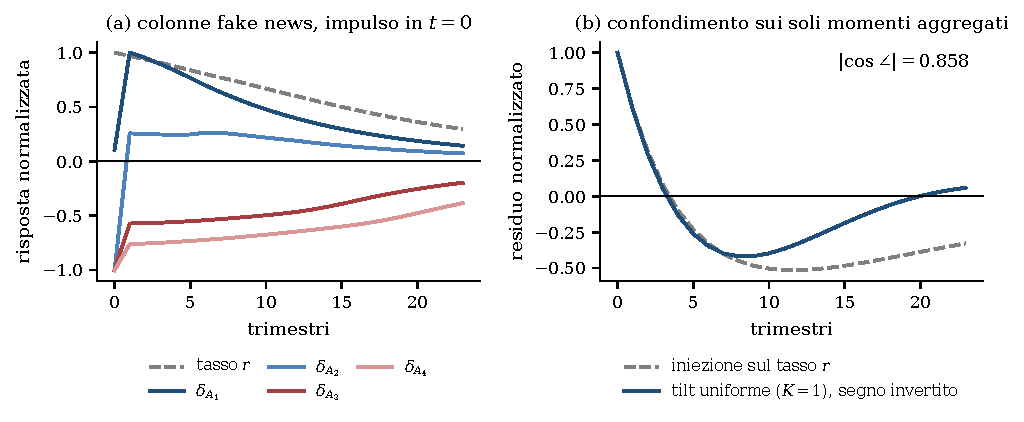
\includegraphics[width=\textwidth]{F1_fakenews.pdf}
\caption{(a) Colonne fake news del Jacobiano a $K=4$ per un impulso unitario in $t=0$, con risposte del consumo aggregato normalizzate al massimo assoluto per il tasso (tratteggio) e per i tilt dei quattro quartili. I profili di $\delta_{A_3}$ e $\delta_{A_4}$ sono quasi proporzionali. (b) Residui non lineari dell'iniezione di tasso e del tilt uniforme ($K=1$), normalizzati e sovrapposti a meno del segno, la cui quasi collinearit\`a ($\lvert\cos\angle\rvert=0{,}858$) costituisce il confondimento fra churn e tasso che fa fallire la risoluzione a $K=1$ sui soli momenti aggregati.}
\label{fig:fakenews}
\end{figure}

\section{Validazioni interne}\label{sec:validazioni}
Quattro verifiche separano ci\`o che \`e esatto da ci\`o che \`e approssimato. La decomposizione (I.11) \`e un'identit\`a algebrica e tiene quindi alla precisione di macchina, sicch\'e sul caso di riferimento lo scarto fra $I^{\mathrm{SSJ}}$, la somma dei contributi di blocco e il calcolo diretto $\tfrac12\Delta\eta^{\star\prime}\Omega^{-1}\Delta\eta^\star$ risulta nullo in doppia precisione. La quadratura di Imhof che implementa la (I.13) \`e validata contro il Monte Carlo nel caso non degenere di riferimento, costituito dall'iniezione aggregata e dalla quota del blocco $A_3$ con $s_{\mathrm{oss}}=0{,}0087$, per il quale il p-value analitico vale $0{,}03708$ contro $0{,}03681$ su $4\times10^5$ estrazioni, uno scarto inferiore all'errore standard Monte Carlo, pari a circa $0{,}0003$. La Figura~\ref{fig:imhof} mostra che l'intera curva $p_k(s)$ si sovrappone alla coda empirica fino al pavimento di risoluzione del campionamento. L'identit\`a di annidamento, secondo cui le colonne del Jacobiano al livello $K$ coincidono con le somme delle colonne ottili, tiene a $2{,}2\times10^{-8}$ in termini relativi, un residuo imputabile alla sola differenziazione numerica. La concordanza, infine, che dopo l'Osservazione 9.5 ha il solo ruolo di misurare la qualit\`a della linearizzazione, restituisce un errore relativo fra residuo non lineare iniettato e previsione lineare $J\eta$ pari allo $0{,}8$ per cento per l'iniezione aggregata e compreso fra il $2{,}0$ e il $4{,}2$ per cento per i tilt, piccolo ma non nullo, e la sua proiezione sulla direzione del residuo costituisce la contaminazione non lineare di cui la Sezione~\ref{sec:limiti} discute il ruolo.

\begin{figure}[t]
\centering
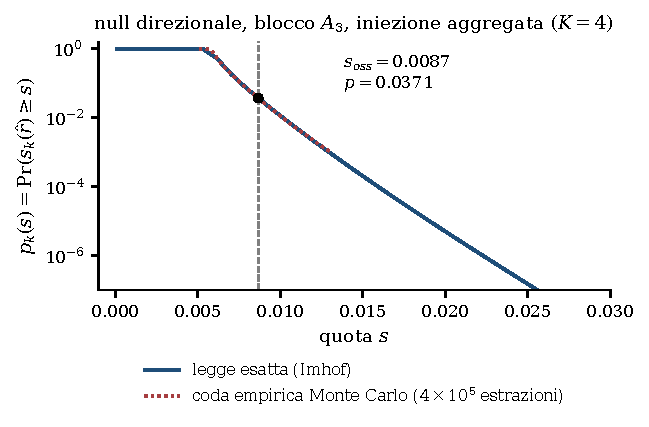
\includegraphics[width=0.62\textwidth]{F2_imhof.pdf}
\caption{Legge esatta del null direzionale (I.13) per la quota del blocco $A_3$ a $K=4$, calcolata per quadratura di Imhof (linea continua), a confronto con la coda empirica su $4\times10^5$ estrazioni del null (punteggiata), con curve indistinguibili fino al pavimento Monte Carlo. Il punto indica la quota osservata nell'iniezione aggregata, $s_{\mathrm{oss}}=0{,}0087$, con $p=0{,}0371$.}
\label{fig:imhof}
\end{figure}

\section{Confusione, molteplicit\`a e la statistica di attribuzione}\label{sec:confusione}
La Figura~\ref{fig:confusione} riporta la matrice di confusione pre-dati della Definizione 10.2 per $K=4$ sui soli momenti aggregati, con le quote $S_{\ell k}$ a sinistra e i p-value $P_{\ell k}$ in scala logaritmica a destra. La struttura \`e coerente con la geometria delle direzioni confondenti, i cui coseni in metrica $Q_{\mathrm{tot}}$ valgono $0{,}997$ fra $v_3$ e $v_4$, $0{,}930$ fra $v_1$ e $v_3$, $0{,}904$ fra $v_1$ e $v_4$ e $0{,}815$ fra $v_{\mathrm{agg}}$ e $v_2$, sicch\'e i due quartili superiori risultano pressoch\'e indistinguibili fra loro e tutti i blocchi patrimoniali si confondono parzialmente con il primo.

Sui p-value marginali si manifesta la patologia anticipata dall'Osservazione 10.6, in forma pi\`u severa del previsto. Nelle righe delle iniezioni forti, cio\`e quelle su $A_1$, $A_3$ e $A_4$, i p-value saturano sotto $10^{-12}$ su tutti i blocchi patrimoniali simultaneamente, e l'$\arg\min_k P_{\ell k}$ della Definizione 10.2 risulta numericamente mal definito, perch\'e la concentrazione appare anomala ovunque e il null direzionale, che riguarda la genericit\`a della direzione del residuo, perde capacit\`a discriminante quando il segnale investe pi\`u blocchi insieme. Il risultato nuovo riguarda il rimedio proposto dalla stessa Osservazione, i contrasti a coppie $\pi_{kj}$, anch'essi di legge weighted-$\chi^2$ e calcolati per quadratura di Imhof. L'attribuzione basata sulla coppia peggiore sbaglia sistematicamente a favore dei blocchi ad alta capacit\`a, assegnando ad $A_4$ le iniezioni su $A_2$ e su $A_3$, e sbaglia anche quando il residuo coincide con la previsione lineare esatta $J\eta$, il che esclude la contaminazione non lineare e riconduce l'errore alla geometria stessa del problema. La ragione \`e meccanica, perch\'e il contrasto $s_k-s_j$ non tiene conto di ci\`o che ciascun blocco \`e in grado di raggiungere, e con $\lambda_{\max}^{(A_4)}=0{,}277$ contro $\lambda_{\max}^{(A_2)}=0{,}022$ il blocco pi\`u capiente assorbe quota anche da residui che non lo riguardano.

La statistica corretta discende dalla Definizione 10.1 come corollario, ed \`e la frazione di capacit\`a utilizzata
\begin{equation}\label{eq:utilization}
u_k\;:=\;\frac{s_k(\hat r)}{\lambda_{\max}^{(k)}}\;\in\;[0,1],
\end{equation}
cio\`e la quota osservata rapportata al massimo del quoziente di Rayleigh generalizzato che il blocco pu\`o raggiungere, massimo che si realizza per $\hat r\propto v_k$. La statistica \`e invariante per riscalamento della geometria del blocco e vale $1$ se e solo se il residuo giace sulla direzione massimamente confondente. Su tutte le iniezioni e su tutti i livelli nei quali esiste una risoluzione, l'attribuzione mediante $\arg\max_k u_k$ \`e corretta nei casi in cui la coppia peggiore fallisce, inclusa l'iniezione debole su $A_2$, per la quale $u_{A_2}=s_{A_2}/0{,}022$ risulta la frazione pi\`u alta, con un margine di $0{,}029$ sul quarto quartile, bench\'e $s_{A_2}$ sia minuscola in valore assoluto. L'emendamento proposto alla Definizione 10.2 separa quindi due giudizi, affidando l'identificazione del blocco all'$\arg\max_k u_k$ e la significativit\`a al p-value (I.13) del solo blocco attribuito, con la condizione $P_{\ell,\hat k(\ell)}\le\alpha$, mentre il margine $u_{(1)}-u_{(2)}$ fra le prime due frazioni di utilizzo diventa la misura naturale della nettezza dell'attribuzione e la grandezza con cui la Sezione~\ref{sec:risoluzione} definisce operativamente la risoluzione.

\begin{figure}[t]
\centering
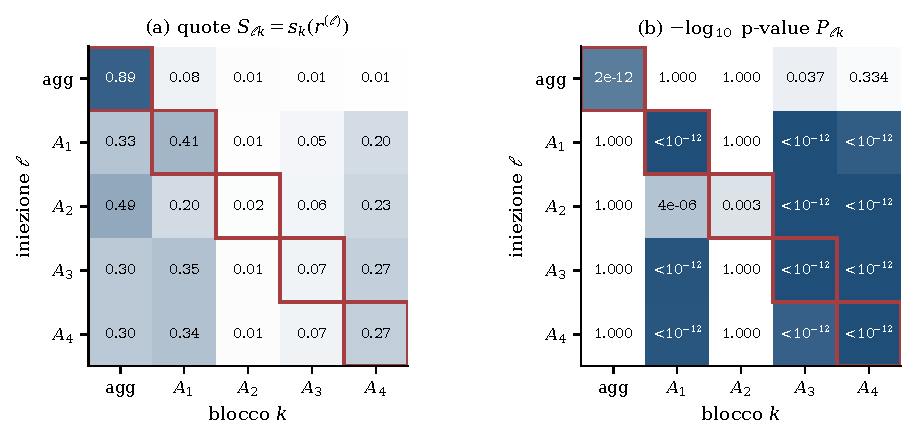
\includegraphics[width=0.95\textwidth]{F3_confusione.pdf}
\caption{Matrice di confusione pre-dati a $K=4$, soli momenti aggregati, $\Neff=8000$, $\rho=128$. (a) Quote $S_{\ell k}=s_k(r^{(\ell)})$ sui residui delle cinque iniezioni, con la diagonale evidenziata. (b) P-value direzionali $P_{\ell k}$ in scala $-\log_{10}$, che nelle righe a segnale forte saturano su pi\`u blocchi simultaneamente e rendono mal definito l'$\arg\min$ (molteplicit\`a, Osservazione 10.6).}
\label{fig:confusione}
\end{figure}

\section{Risoluzione della famiglia annidata e dipendenza dai momenti}\label{sec:risoluzione}
La Tabella~\ref{tab:risoluzione} e la Figura~\ref{fig:risoluzione} riportano il verdetto di risoluzione lungo la famiglia annidata per i due insiemi di momenti, considerando risolto un livello quando la frazione di utilizzo attribuisce correttamente tutte le sue iniezioni, e indicando il margine minimo e il peggior p-value del blocco vero.

Sui soli momenti aggregati l'esito non \`e monotono, e in questo consiste il quarto risultato sostanziale. Il livello $K=1$ fallisce, perch\'e il tilt uniforme viene attribuito al blocco aggregato con un margine di $0{,}443$, dato che sul consumo aggregato un aumento generalizzato del churn \`e quasi collineare a uno shock di tasso, come anticipato nel pannello (b) della Figura~\ref{fig:fakenews}. Si tratta del confondimento economicamente pi\`u rilevante dell'esercizio, fra la dinamica del reddito idiosincratico e il canale intertemporale del tasso, e una diagnostica condotta sui soli aggregati non ha modo di rilevarlo, giacch\'e l'attribuzione errata avviene con un margine ampio. Il livello $K=2$ risolve con margine $0{,}096$, poich\'e la suddivisione della popolazione in due met\`a patrimoniali basta a separare il churn dal tasso, dato che i tilt sulle due met\`a lasciano sul consumo aggregato impronte di profilo diverso. Il livello $K=4$ \`e formalmente risolto ma prossimo alla degenerazione, con un margine minimo di $4{,}4\times10^{-6}$ interamente concentrato sulla coppia formata da $A_3$ e $A_4$, i cui coni di confondimento quasi coincidono, come indica un coseno di $0{,}997$. Il livello $K=8$ fallisce infine con inversioni multiple fra ottili adiacenti. La risoluzione della famiglia, nel senso della Definizione 10.2, \`e dunque $K=2$, e la non monotonia impone di leggere la Definizione con cura. L'insieme dei livelli risolventi non \`e un segmento iniziale della famiglia, sicch\'e il criterio d'arresto del raffinamento richiede la scansione dell'intera famiglia, e un fallimento al livello pi\`u grossolano costituisce esso stesso un'informazione, poich\'e segnala che la partizione banale proietta il livello idiosincratico su un'unica direzione aggregata gi\`a occupata dal tasso.

L'ampliamento dell'insieme dei momenti scioglie il quadro. Aggiungendo dodici momenti distributivi, ossia la deviazione percentuale del consumo della met\`a meno ricca della popolazione per ricchezza di inizio periodo, con massa $0{,}482$ e orizzonte di dodici trimestri, e ricalibrando $\rho=179{,}4$ allo stesso fit medio, il livello $K=1$ si sblocca con margine $0{,}792$ e p-value del blocco vero pari a $2{,}9\times10^{-10}$. I momenti del gruppo meno ricco rompono la collinearit\`a fra churn e tasso perch\'e su quel gruppo i due meccanismi si muovono nello stesso verso, con un coseno di $0{,}70$, mentre sul consumo aggregato si muovono in verso opposto, sicch\'e nessuna riscalatura di un meccanismo pu\`o imitare l'altro su entrambi gli insiemi di momenti. Il margine a $K=2$ quasi quadruplica, salendo a $0{,}355$, il livello $K=4$ passa dalla quasi degenerazione a una risoluzione solida con margine $0{,}092$, e su questi momenti anche l'attribuzione basata sulla coppia peggiore torna corretta fino a $K=4$, mentre il livello $K=8$ resta non risolto, con un margine di $0{,}0056$, circa ventiquattro volte pi\`u ampio. Coerentemente, la stessa iniezione porta pi\`u informazione, e per quella aggregata $I^{\mathrm{SSJ}}$ sale da $2{,}09$ a $4{,}14$ mentre la $\DEP$ scende da $0{,}154$ a $0{,}075$.

Ne discende un emendamento, secondo cui la risoluzione \`e una propriet\`a congiunta della coppia formata da dizionario e momenti. La Definizione 10.2 va indicizzata a entrambi gli argomenti, e l'Osservazione 9.5, che fissa il criterio d'arresto del raffinamento della sieve, va letta condizionatamente all'insieme dei momenti vincolati. La direzione inversa \`e altrettanto utile, perch\'e a dizionario fissato la coppia $(S,P)$ pre-dati diventa un criterio di valore diagnostico dei momenti, che indica quali target aggiungere per separare i blocchi confusi prima di stimare alcunch\'e, e nel caso in esame un solo blocco di momenti distributivi porta da $K=2$ a $K=4$ la partizione pi\`u fine risolta con margine apprezzabile.

\begin{table}[t]
\centering\small
\caption{Verdetto di risoluzione per livello della famiglia annidata con attribuzione per frazione di capacit\`a utilizzata \eqref{eq:utilization}. L'esito \`e positivo quando tutte le iniezioni del livello sono attribuite correttamente, e sono riportati il margine minimo $u_{(1)}-u_{(2)}$ e il peggior p-value del blocco vero, con $\Neff=8000$, $\rho=128$ per i soli aggregati e $\rho=179{,}4$ per i momenti aumentati, e fit medio $0{,}95$ a $K=4$ in entrambi i casi.}
\label{tab:risoluzione}
\begin{tabular}{lcccccc}
\toprule
& \multicolumn{3}{c}{soli aggregati ($H=24$)} & \multicolumn{3}{c}{aumentati ($H=24+12$)}\\
\cmidrule(lr){2-4}\cmidrule(lr){5-7}
livello & esito & margine & $\max_\ell P_{\ell,k(\ell)}$ & esito & margine & $\max_\ell P_{\ell,k(\ell)}$\\
\midrule
$K=1$ & no & $0{,}443$ & $\approx1$ & s\`i & $0{,}792$ & $2{,}9\times10^{-10}$\\
$K=2$ & s\`i & $0{,}096$ & $9{,}3\times10^{-14}$ & s\`i & $0{,}355$ & $1{,}7\times10^{-6}$\\
$K=4$ & s\`i & $4{,}4\times10^{-6}$ & $2{,}8\times10^{-3}$ & s\`i & $0{,}092$ & $4{,}1\times10^{-6}$\\
$K=8$ & no & $2{,}4\times10^{-4}$ & $\approx1$ & no & $5{,}6\times10^{-3}$ & $2{,}1\times10^{-4}$\\
\bottomrule
\end{tabular}
\end{table}

\begin{figure}[t]
\centering
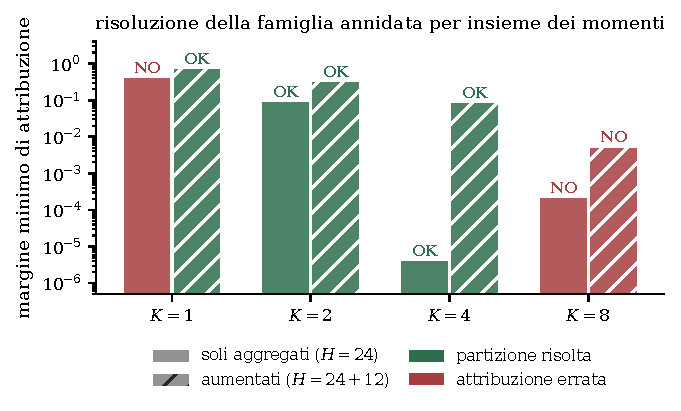
\includegraphics[width=0.72\textwidth]{F4_risoluzione.pdf}
\caption{Margine minimo di attribuzione in scala logaritmica per livello della famiglia annidata e per insieme dei momenti, con il colore a indicare l'esito. La risoluzione non \`e monotona nel raffinamento, dato che sui soli aggregati $K=1$ fallisce e $K=2$ risolve, ed \`e crescente nell'insieme dei momenti, poich\'e dodici momenti della met\`a meno ricca della popolazione sbloccano $K=1$ e portano a $K=4$ la partizione pi\`u fine risolta con margine apprezzabile.}
\label{fig:risoluzione}
\end{figure}

\section{Stabilit\`a C3 in forma analitica}\label{sec:c3}
Il controllo C3, nella forma riallocata dell'Osservazione 10.5, consiste nel ricalcolo in forma chiusa della coppia $(M,\{Q_k\})$ con il peso $\rho$ riscalato. La Tabella~\ref{tab:c3} riporta fit e quote per l'iniezione aggregata a $K=4$ con pesi pari a $0{,}1\,\rho$, $\rho$ e $10\,\rho$. Fra $\rho$ e $10\,\rho$ le quote variano al pi\`u di circa un centesimo, con la quota aggregata che passa da $0{,}891$ a $0{,}902$, mentre a $0{,}1\,\rho$ il fit scende a $0{,}69$ e la quota aggregata a $0{,}80$, e la parte rilasciata viene assorbita quasi interamente dal primo quartile. La riallocazione fra fit e attribuzione si muove quindi nella direzione attesa, senza ribaltamenti dell'ordinamento.

\begin{table}[t]
\centering\small
\caption{Controllo C3 analitico per l'iniezione aggregata, $K=4$, soli momenti aggregati, $\Neff=8000$.}
\label{tab:c3}
\begin{tabular}{lcccccc}
\toprule
peso & fit & agg & $A_1$ & $A_2$ & $A_3$ & $A_4$\\
\midrule
$0{,}1\,\rho$ & $0{,}691$ & $0{,}797$ & $0{,}164$ & $0{,}010$ & $0{,}013$ & $0{,}015$\\
$\rho$ & $0{,}919$ & $0{,}891$ & $0{,}080$ & $0{,}014$ & $0{,}009$ & $0{,}006$\\
$10\,\rho$ & $0{,}988$ & $0{,}902$ & $0{,}067$ & $0{,}016$ & $0{,}008$ & $0{,}007$\\
\bottomrule
\end{tabular}
\end{table}

\section{Limiti dell'esercizio e implicazioni per la nota}\label{sec:limiti}
Cinque limiti vanno dichiarati, in ordine di sostanza. Il primo \`e l'equilibrio parziale, poich\'e le colonne fake news incorporano l'anticipazione comportamentale dei sentieri annunciati senza alcuna risposta dei prezzi, sicch\'e la separazione fra $\Omega$ e $J$ dell'Osservazione 9.4 \`e esercitata nella sola met\`a diretta e il contenuto di equilibrio generale di $J$ resta da verificare nel modello HANK completo. Il secondo riguarda la natura del tilt, che modificando in modo simmetrico le due probabilit\`a di transizione altera insieme la persistenza del reddito e, attraverso la composizione della regione per stato di reddito, il reddito atteso, sicch\'e la separazione fra correzione della propagazione e correzione del rischio richiede due tilt per regione, uno asimmetrico che sposta il reddito atteso e uno che ne modifica la persistenza a reddito atteso invariato. Il terzo \`e la componente del residuo non lineare esterna allo span lineare, che la concordanza quantifica fra l'uno e il quattro per cento e che la proiezione attribuisce comunque ai blocchi, e che nei casi al limite, come quello della coppia formata da $A_3$ e $A_4$ a $K=4$, \`e dello stesso ordine del margine, tanto che la verit\`a si recupera soltanto ampliando i momenti. Il quarto \`e l'orizzonte di troncamento $T=40$, che taglia le code delle colonne fake news pi\`u persistenti con un errore che la concordanza ingloba senza isolarlo, mentre il quindi concerne $\Neff$, che \`e dichiarato e non stimato, sicch\'e capacit\`a, confusione e risoluzione dipendono dal rapporto di costo fra i livelli e la Tabella~\ref{tab:capacita} va letta come analisi di sensitivit\`a obbligatoria del disegno.

Le implicazioni per la nota e per l'integrazione si riassumono in quattro emendamenti puntuali, tutti gi\`a argomentati. Alla (I.10) si aggiunge il fattore $\Neff$ come nella \eqref{eq:pinningN}, con l'interpretazione di statistica del disegno empirico da dichiarare accanto ad $\alpha$ e $\rho$. All'Osservazione 10.6 si aggiunge l'avvertenza che i contrasti a coppie, pur risolvendo la molteplicit\`a formale, ereditano la distorsione verso i blocchi ad alta capacit\`a e vanno quindi esclusi come regola di attribuzione. Nella Definizione 10.2 l'identificazione passa dall'$\arg\min_k P_{\ell k}$ all'$\arg\max_k u_k$, con $u_k=s_k/\lambda_{\max}^{(k)}$, riservando il p-value al giudizio di significativit\`a sul blocco attribuito e il margine di utilizzo alla misura della nettezza. La stessa Definizione, e con essa il criterio d'arresto dell'Osservazione 9.5, vanno infine indicizzati alla coppia formata da dizionario e momenti, con la lettura duale della matrice di confusione come criterio di valore diagnostico dei momenti, che di quella indicizzazione costituisce il dividendo operativo. Gli emendamenti riguardano il protocollo e lasciano intatti i teoremi dell'integrazione, che l'esercizio conferma alla precisione di macchina.

\bigskip
\noindent\emph{Replicabilit\`a.} L'intero esercizio \`e riprodotto dai file Python del repository, ossia \texttt{model.py}, che contiene modello, dizionario e Jacobiano, \texttt{entropic.py}, che contiene proiezione, quote, quadratura di Imhof, capacit\`a e confusione, \texttt{run\_all.py} per la famiglia annidata sui momenti aggregati, \texttt{run\_micro.py} per i momenti aumentati e \texttt{figures.py} per le figure, eseguiti in sequenza dal comando \texttt{make} in meno di un minuto su una macchina ordinaria, senza dipendenze oltre NumPy, SciPy e Matplotlib.

\end{document}
